% \chapter{Determining how to parse a formal language}

\section{Introduction}

\newpage
\section{Language Parsing Design}
\subsection{Determining how to parse the syntax of a language}
A formal language is defined as a set of strings of symbols for use in situations where a natural language(\textit{English}) isn't suitable eg. Mathematics, and Computer programming. Where each symbol has precise semantic, and syntactic relation to each other. Writing formal grammar rules uses a set of finite ``\textit{productions}''. Productions, are rules that signify substitution of Symbols within a string, there are typically three symbols when writing productions in formal grammars as seen in figure \ref{fig:formalGrammar}. Productions rules are used to take strings, and convert them into parse trees, which are a hierarchy of tokens that can be used by the \compiler{}. The \textit{|} symbol is just a grouping of rules applying to the same rule so $A \rightarrow a | aA$ is the same as $$A &\rightarrow a \\ A &\rightarrow aA$$

\begin{figure}[ht!]
    \begin{align*}
    S_s &\rightarrow AB\ |\ CC \\
    A &\rightarrow a\ |\ aA \\
    B &\rightarrow bc\ |\ bBc \\
    D &\rightarrow ab\ |\ aDb \\
    C &\rightarrow c\ |\ cC \\
    \end{align*}
    \caption{Formal grammar syntax, example from \cite{ParseTech}}
    \label{fig:formalGrammar}
\end{figure}
\subsubsection{Grammar definitions}
\begin{description}
    \item[\textit{Terminal Symbols}] Symbols which cannot be substituted any further, an example of this in programming languages is literal characters, or a single number digit. Terminal symbols are represented by lowercase letters.
    
    \item[\textit{Nonterminal Symbols}] Symbols which can be reduced further using productions. For example as in \ref{fig:formalGrammar} $A \rightarrow a\ |\ aA$ is a nonterminal rule, as \textit{A} needs to be substituted into either \textit{a}, or \textit{aA}. Nonterminal symbols are represented by uppercase letters.

    \item[\textit{Start Symbol}] is a special Nonterminal symbol signifying the start of a string. Start symbols are represented by a uppercase S, or an Uppercase S with a subscript s eg. $S_s$, in order to signify it is different from a Nonterminal \textit{S} symbol.
\end{description}

In \autocite{Chomsky} he defined what is now known as \textit{Chomsky-Schützenberger hierarchy}, which defines formal languages into four types(Type 0 - 4). As shown in Figure \ref{fig:Chomsky} each type is a subset of the previous. All of Type 4, can be a Type 0, but not all of Type 0 can be Type 4, so multiple rules can describe the same language depending on it's syntax.
\begin{figure}[ht!]
    \centerline{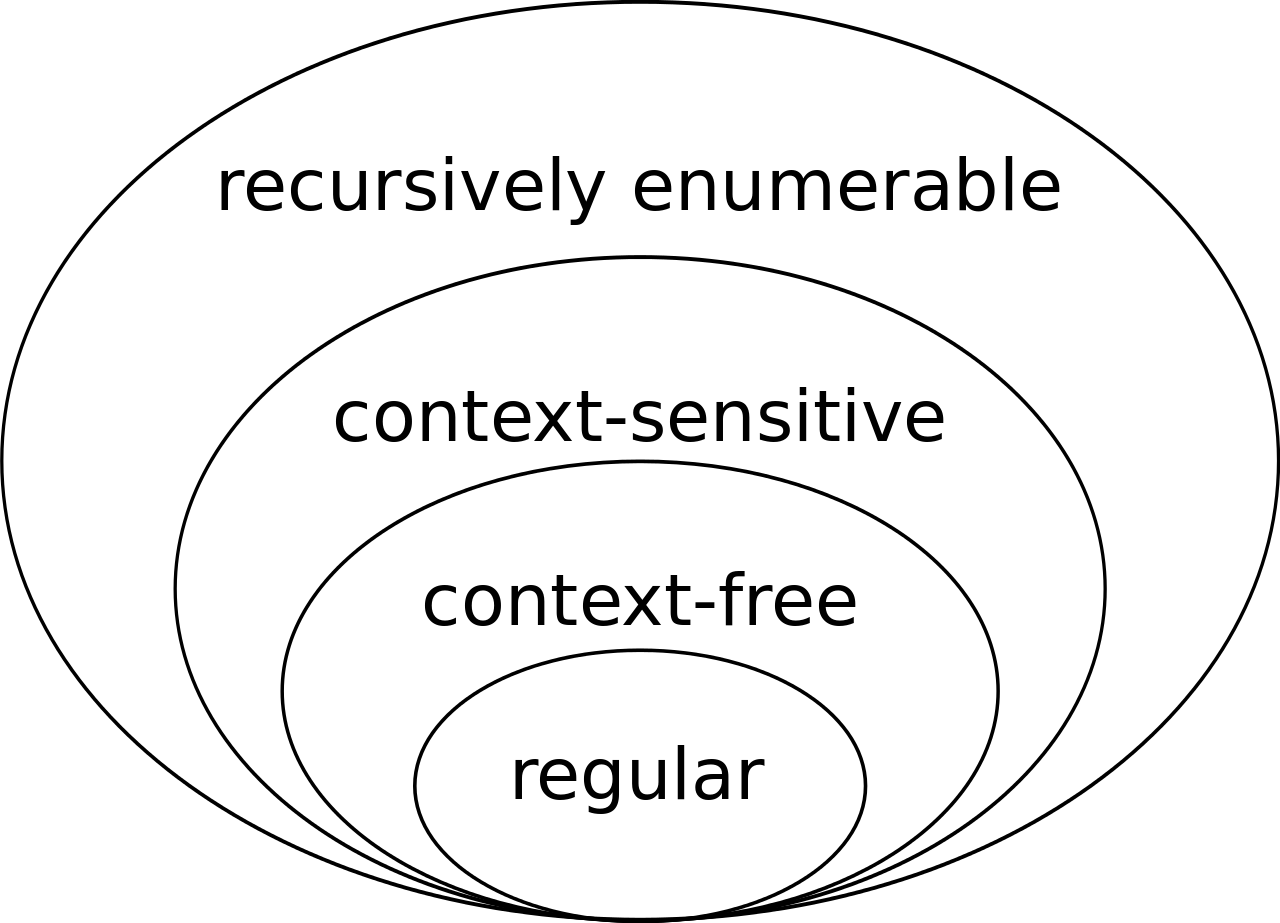
\includegraphics[width=0.5\linewidth]{img/Chomsky.png}}
    \caption{Chomsky-Schützenberger hierarchy, by J. Finkelstein}
    \label{fig:Chomsky}
\end{figure}
\subsubsection{Language types}
\begin{description}
    \item[Type 0] Also known as \textit{phase structure} languages. This is the the parent of all following languages. Every language in the Chomsky hierarchy is also a phase structure. Phase structure is a generalised, and can have unclear hierarchy, due to it's lack of limitations.
    \item[Type 1] Also known as \textit{context-sensitive} languages. Meaning only one of the nonterminal characters on the left hand side can be replaced. This allows for a much more clear hierarchy within the parse tree.
    \item[Type 2] Also known as \textit{context-free} languages. context-free is similar to context sensitive, except there is always only one Nonterminal Symbol on the left hand side. This prevents children in the parse tree to have siblings, providing a \textit{pure} hierarchy. This is a the type most programming languages fall under.
    \item[Type 3]  Also known as \textit{regular} languages. Regular languages are languages defined by \textit{regular expressions} rather than regular grammar like seen previously.
\end{description}

\autocite{ParseTech} posits that 



\newpage
\section{Conclusion}